\documentclass{extbook}[14pt]
\usepackage{multicol, enumerate, enumitem, hyperref, color, soul, setspace, parskip, fancyhdr, amssymb, amsthm, amsmath, latexsym, units, mathtools}
\everymath{\displaystyle}
\usepackage[headsep=0.5cm,headheight=0cm, left=1 in,right= 1 in,top= 1 in,bottom= 1 in]{geometry}
\usepackage{dashrule}  % Package to use the command below to create lines between items
\newcommand{\litem}[1]{\item #1

\rule{\textwidth}{0.4pt}}
\pagestyle{fancy}
\lhead{}
\chead{Answer Key for Makeup Progress Quiz 2 Version A}
\rhead{}
\lfoot{5763-3522}
\cfoot{}
\rfoot{Spring 2021}
\begin{document}
\textbf{This key should allow you to understand why you choose the option you did (beyond just getting a question right or wrong). \href{https://xronos.clas.ufl.edu/mac1105spring2020/courseDescriptionAndMisc/Exams/LearningFromResults}{More instructions on how to use this key can be found here}.}

\textbf{If you have a suggestion to make the keys better, \href{https://forms.gle/CZkbZmPbC9XALEE88}{please fill out the short survey here}.}

\textit{Note: This key is auto-generated and may contain issues and/or errors. The keys are reviewed after each exam to ensure grading is done accurately. If there are issues (like duplicate options), they are noted in the offline gradebook. The keys are a work-in-progress to give students as many resources to improve as possible.}

\rule{\textwidth}{0.4pt}

\begin{enumerate}\litem{
Construct the lowest-degree polynomial given the zeros below. Then, choose the intervals that contain the coefficients of the polynomial in the form $ax^3+bx^2+cx+d$.
\[ \frac{4}{5}, \frac{3}{2}, \text{ and } \frac{7}{4} \]The solution is \( 40x^{3} -162 x^{2} +209 x -84 \), which is option B.\begin{enumerate}[label=\Alph*.]
\item \( a \in [38, 45], b \in [-98, -95], c \in [-1, 4], \text{ and } d \in [76, 87] \)

$40x^{3} -98 x^{2} +x + 84$, which corresponds to multiplying out $(5x + 4)(2x -3)(4x -7)$.
\item \( a \in [38, 45], b \in [-167, -157], c \in [204, 222], \text{ and } d \in [-85, -78] \)

* $40x^{3} -162 x^{2} +209 x -84$, which is the correct option.
\item \( a \in [38, 45], b \in [22, 24], c \in [-118, -107], \text{ and } d \in [-85, -78] \)

$40x^{3} +22 x^{2} -113 x -84$, which corresponds to multiplying out $(5x + 4)(2x + 3)(4x -7)$.
\item \( a \in [38, 45], b \in [-167, -157], c \in [204, 222], \text{ and } d \in [76, 87] \)

$40x^{3} -162 x^{2} +209 x + 84$, which corresponds to multiplying everything correctly except the constant term.
\item \( a \in [38, 45], b \in [158, 163], c \in [204, 222], \text{ and } d \in [76, 87] \)

$40x^{3} +162 x^{2} +209 x + 84$, which corresponds to multiplying out $(5x + 4)(2x + 3)(4x + 7)$.
\end{enumerate}

\textbf{General Comment:} To construct the lowest-degree polynomial, you want to multiply out $(5x -4)(2x -3)(4x -7)$
}
\litem{
Construct the lowest-degree polynomial given the zeros below. Then, choose the intervals that contain the coefficients of the polynomial in the form $x^3+bx^2+cx+d$.
\[ -2 + 2 i \text{ and } 2 \]The solution is \( x^{3} +2 x^{2} -16 \), which is option A.\begin{enumerate}[label=\Alph*.]
\item \( b \in [1.07, 2.48], c \in [-1.6, 0.7], \text{ and } d \in [-21, -13] \)

* $x^{3} +2 x^{2} -16$, which is the correct option.
\item \( b \in [-3.13, -1.69], c \in [-1.6, 0.7], \text{ and } d \in [13, 22] \)

$x^{3} -2 x^{2} + 16$, which corresponds to multiplying out $(x-(-2 + 2 i))(x-(-2 - 2 i))(x + 2)$.
\item \( b \in [0.96, 1.95], c \in [-5.5, -3.4], \text{ and } d \in [4, 9] \)

$x^{3} + x^{2} -4 x + 4$, which corresponds to multiplying out $(x -2)(x -2)$.
\item \( b \in [0.96, 1.95], c \in [-1.6, 0.7], \text{ and } d \in [-9, -3] \)

$x^{3} + x^{2} -4$, which corresponds to multiplying out $(x + 2)(x -2)$.
\item \( \text{None of the above.} \)

This corresponds to making an unanticipated error or not understanding how to use nonreal complex numbers to create the lowest-degree polynomial. If you chose this and are not sure what you did wrong, please contact the coordinator for help.
\end{enumerate}

\textbf{General Comment:} Remember that the conjugate of $a+bi$ is $a-bi$. Since these zeros always come in pairs, we need to multiply out $(x-(-2 + 2 i))(x-(-2 - 2 i))(x-(2))$.
}
\litem{
Which of the following equations \textit{could} be of the graph presented below?

\begin{center}
    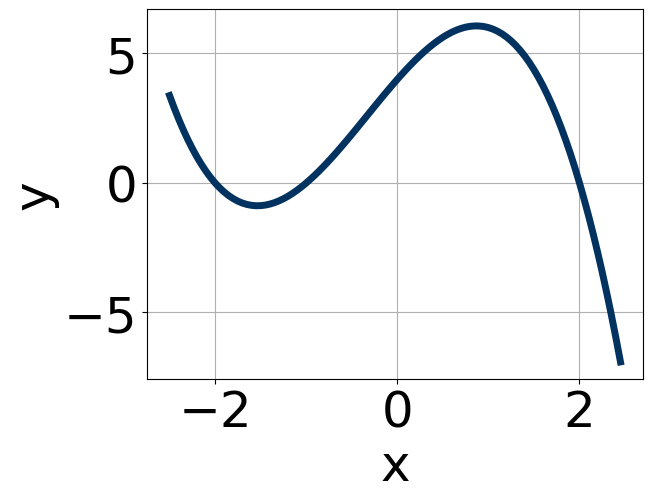
\includegraphics[width=0.5\textwidth]{../Figures/polyGraphToFunctionA.png}
\end{center}


The solution is \( -14(x + 1)^{11} (x - 2)^{9} (x + 2)^{7} \), which is option B.\begin{enumerate}[label=\Alph*.]
\item \( 15(x + 1)^{9} (x - 2)^{5} (x + 2)^{7} \)

This corresponds to the leading coefficient being the opposite value than it should be.
\item \( -14(x + 1)^{11} (x - 2)^{9} (x + 2)^{7} \)

* This is the correct option.
\item \( 19(x + 1)^{6} (x - 2)^{5} (x + 2)^{9} \)

The factor $(x + 1)$ should have an odd power and the leading coefficient should be the opposite sign.
\item \( -13(x + 1)^{10} (x - 2)^{10} (x + 2)^{11} \)

The factors $-1$ and $2$ have have been odd power.
\item \( -8(x + 1)^{10} (x - 2)^{7} (x + 2)^{9} \)

The factor $-1$ should have been an odd power.
\end{enumerate}

\textbf{General Comment:} General Comments: Draw the x-axis to determine which zeros are touching (and so have even multiplicity) or cross (and have odd multiplicity).
}
\litem{
Describe the zero behavior of the zero $x = 9$ of the polynomial below.
\[ f(x) = -2(x + 9)^{2}(x - 9)^{7}(x - 4)^{5}(x + 4)^{9} \]The solution is the graph below, which is option A.
\begin{center}
    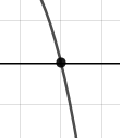
\includegraphics[width=0.3\textwidth]{../Figures/polyZeroBehaviorCopyAA.png}
\end{center}\begin{enumerate}[label=\Alph*.]
\begin{multicols}{2}
\item 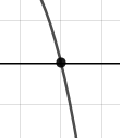
\includegraphics[width = 0.3\textwidth]{../Figures/polyZeroBehaviorCopyAA.png}
\item 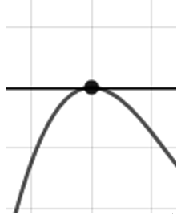
\includegraphics[width = 0.3\textwidth]{../Figures/polyZeroBehaviorCopyBA.png}
\item 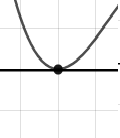
\includegraphics[width = 0.3\textwidth]{../Figures/polyZeroBehaviorCopyCA.png}
\item 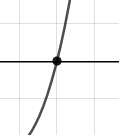
\includegraphics[width = 0.3\textwidth]{../Figures/polyZeroBehaviorCopyDA.png}
\end{multicols}\item None of the above.\end{enumerate}
\textbf{General Comment:} You will need to sketch the entire graph, then zoom in on the zero the question asks about.
}
\litem{
Describe the zero behavior of the zero $x = 6$ of the polynomial below.
\[ f(x) = -7(x + 2)^{4}(x - 2)^{2}(x + 6)^{5}(x - 6)^{4} \]The solution is the graph below, which is option B.
\begin{center}
    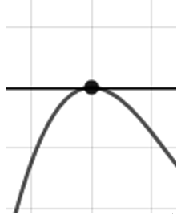
\includegraphics[width=0.3\textwidth]{../Figures/polyZeroBehaviorBA.png}
\end{center}\begin{enumerate}[label=\Alph*.]
\begin{multicols}{2}
\item 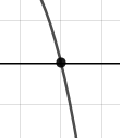
\includegraphics[width = 0.3\textwidth]{../Figures/polyZeroBehaviorAA.png}
\item 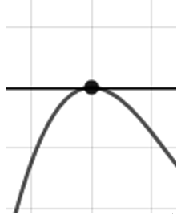
\includegraphics[width = 0.3\textwidth]{../Figures/polyZeroBehaviorBA.png}
\item 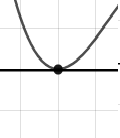
\includegraphics[width = 0.3\textwidth]{../Figures/polyZeroBehaviorCA.png}
\item 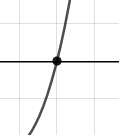
\includegraphics[width = 0.3\textwidth]{../Figures/polyZeroBehaviorDA.png}
\end{multicols}\item None of the above.\end{enumerate}
\textbf{General Comment:} You will need to sketch the entire graph, then zoom in on the zero the question asks about.
}
\litem{
Construct the lowest-degree polynomial given the zeros below. Then, choose the intervals that contain the coefficients of the polynomial in the form $x^3+bx^2+cx+d$.
\[ -5 - 2 i \text{ and } 2 \]The solution is \( x^{3} +8 x^{2} +9 x -58 \), which is option D.\begin{enumerate}[label=\Alph*.]
\item \( b \in [-12, -4], c \in [4.8, 9.5], \text{ and } d \in [58, 60] \)

$x^{3} -8 x^{2} +9 x + 58$, which corresponds to multiplying out $(x-(-5 - 2 i))(x-(-5 + 2 i))(x + 2)$.
\item \( b \in [1, 4], c \in [-7.7, 1.2], \text{ and } d \in [-5, 3] \)

$x^{3} + x^{2} -4$, which corresponds to multiplying out $(x + 2)(x -2)$.
\item \( b \in [1, 4], c \in [2.7, 3.6], \text{ and } d \in [-11, -8] \)

$x^{3} + x^{2} +3 x -10$, which corresponds to multiplying out $(x + 5)(x -2)$.
\item \( b \in [3, 14], c \in [4.8, 9.5], \text{ and } d \in [-63, -54] \)

* $x^{3} +8 x^{2} +9 x -58$, which is the correct option.
\item \( \text{None of the above.} \)

This corresponds to making an unanticipated error or not understanding how to use nonreal complex numbers to create the lowest-degree polynomial. If you chose this and are not sure what you did wrong, please contact the coordinator for help.
\end{enumerate}

\textbf{General Comment:} Remember that the conjugate of $a+bi$ is $a-bi$. Since these zeros always come in pairs, we need to multiply out $(x-(-5 - 2 i))(x-(-5 + 2 i))(x-(2))$.
}
\litem{
Construct the lowest-degree polynomial given the zeros below. Then, choose the intervals that contain the coefficients of the polynomial in the form $ax^3+bx^2+cx+d$.
\[ 4, \frac{7}{3}, \text{ and } \frac{1}{5} \]The solution is \( 15x^{3} -98 x^{2} +159 x -28 \), which is option D.\begin{enumerate}[label=\Alph*.]
\item \( a \in [11, 20], b \in [13, 26], c \in [-145, -141], \text{ and } d \in [21, 36] \)

$15x^{3} +22 x^{2} -145 x + 28$, which corresponds to multiplying out $(x + 4)(3x -7)(5x -1)$.
\item \( a \in [11, 20], b \in [98, 105], c \in [158, 162], \text{ and } d \in [21, 36] \)

$15x^{3} +98 x^{2} +159 x + 28$, which corresponds to multiplying out $(x + 4)(3x + 7)(5x + 1)$.
\item \( a \in [11, 20], b \in [-101, -96], c \in [158, 162], \text{ and } d \in [21, 36] \)

$15x^{3} -98 x^{2} +159 x + 28$, which corresponds to multiplying everything correctly except the constant term.
\item \( a \in [11, 20], b \in [-101, -96], c \in [158, 162], \text{ and } d \in [-31, -27] \)

* $15x^{3} -98 x^{2} +159 x -28$, which is the correct option.
\item \( a \in [11, 20], b \in [89, 93], c \in [115, 123], \text{ and } d \in [-31, -27] \)

$15x^{3} +92 x^{2} +121 x -28$, which corresponds to multiplying out $(x + 4)(3x + 7)(5x -1)$.
\end{enumerate}

\textbf{General Comment:} To construct the lowest-degree polynomial, you want to multiply out $(x -4)(3x -7)(5x -1)$
}
\litem{
Describe the end behavior of the polynomial below.
\[ f(x) = -3(x + 2)^{5}(x - 2)^{6}(x + 6)^{4}(x - 6)^{6} \]The solution is the graph below, which is option A.
\begin{center}
    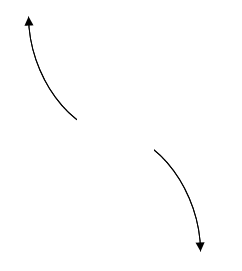
\includegraphics[width=0.3\textwidth]{../Figures/polyEndBehaviorCopyAA.png}
\end{center}\begin{enumerate}[label=\Alph*.]
\begin{multicols}{2}
\item 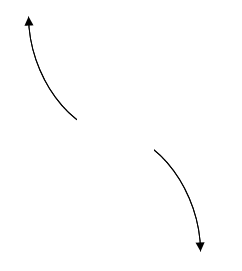
\includegraphics[width = 0.3\textwidth]{../Figures/polyEndBehaviorCopyAA.png}
\item 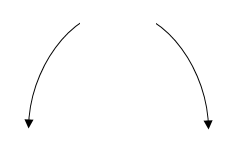
\includegraphics[width = 0.3\textwidth]{../Figures/polyEndBehaviorCopyBA.png}
\item 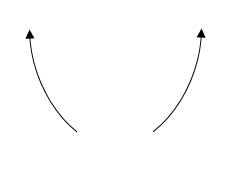
\includegraphics[width = 0.3\textwidth]{../Figures/polyEndBehaviorCopyCA.png}
\item 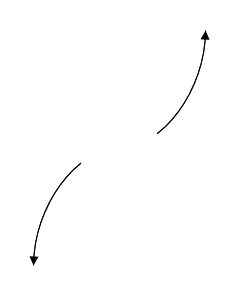
\includegraphics[width = 0.3\textwidth]{../Figures/polyEndBehaviorCopyDA.png}
\end{multicols}\item None of the above.\end{enumerate}
\textbf{General Comment:} Remember that end behavior is determined by the leading coefficient AND whether the \textbf{sum} of the multiplicities is positive or negative.
}
\litem{
Which of the following equations \textit{could} be of the graph presented below?

\begin{center}
    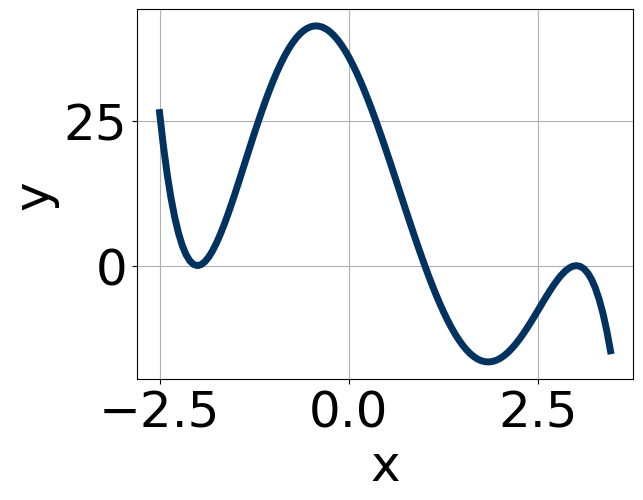
\includegraphics[width=0.5\textwidth]{../Figures/polyGraphToFunctionCopyA.png}
\end{center}


The solution is \( -17(x - 3)^{8} (x + 2)^{4} (x - 1)^{11} \), which is option D.\begin{enumerate}[label=\Alph*.]
\item \( -5(x - 3)^{4} (x + 2)^{5} (x - 1)^{4} \)

The factor $(x + 2)$ should have an even power and the factor $(x - 1)$ should have an odd power.
\item \( -8(x - 3)^{10} (x + 2)^{5} (x - 1)^{9} \)

The factor $(x + 2)$ should have an even power.
\item \( 4(x - 3)^{10} (x + 2)^{8} (x - 1)^{7} \)

This corresponds to the leading coefficient being the opposite value than it should be.
\item \( -17(x - 3)^{8} (x + 2)^{4} (x - 1)^{11} \)

* This is the correct option.
\item \( 20(x - 3)^{10} (x + 2)^{6} (x - 1)^{6} \)

The factor $(x - 1)$ should have an odd power and the leading coefficient should be the opposite sign.
\end{enumerate}

\textbf{General Comment:} General Comments: Draw the x-axis to determine which zeros are touching (and so have even multiplicity) or cross (and have odd multiplicity).
}
\litem{
Describe the end behavior of the polynomial below.
\[ f(x) = -8(x + 2)^{2}(x - 2)^{7}(x - 8)^{2}(x + 8)^{2} \]The solution is the graph below, which is option A.
\begin{center}
    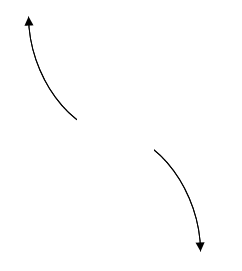
\includegraphics[width=0.3\textwidth]{../Figures/polyEndBehaviorAA.png}
\end{center}\begin{enumerate}[label=\Alph*.]
\begin{multicols}{2}
\item 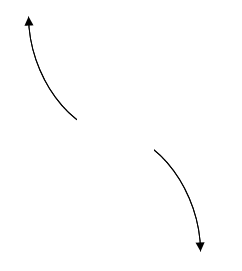
\includegraphics[width = 0.3\textwidth]{../Figures/polyEndBehaviorAA.png}
\item 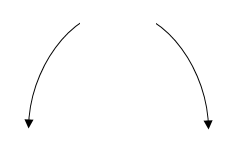
\includegraphics[width = 0.3\textwidth]{../Figures/polyEndBehaviorBA.png}
\item 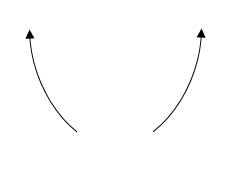
\includegraphics[width = 0.3\textwidth]{../Figures/polyEndBehaviorCA.png}
\item 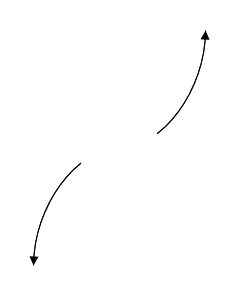
\includegraphics[width = 0.3\textwidth]{../Figures/polyEndBehaviorDA.png}
\end{multicols}\item None of the above.\end{enumerate}
\textbf{General Comment:} Remember that end behavior is determined by the leading coefficient AND whether the \textbf{sum} of the multiplicities is positive or negative.
}
\end{enumerate}

\end{document}